\documentclass{article}

\usepackage{explorations}

\title{(1.0.0.1) Introduction}
\module{Module 1}
\course{Explorations 1}

\begin{document}
\section*{Module 1: Overview and Expectations}

\begin{wrapfigure}[10]{R}{0.25\textwidth}
  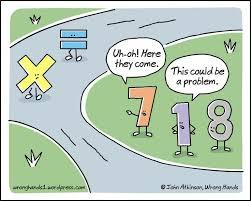
\includegraphics[width=0.25\textwidth]{numbers-walking.jpg}
\end{wrapfigure}
Our first module introduces you to a seemingly unrelated set of activities that are intended to challenge your thinking, as well as the way you process information.  This module intends to amplify your perspective on how to analyze and dissect multiple types of problems.  You will be engaging in activities that begin to develop in your mathematical thinking.  These activities range from mathematically historic forms of computations, to developing a sense and understanding of numbers, their magnitudes, how to represent them and how the differences in number representations and organization will assist in effectively analyzing and solving problems.  

You will get an introduction of the differences between the various types of numbers and you will begin to develop an appreciation and a sense of the structure of the system of numbers.

You will be using this newly discovered structure of the number system to attempt at recognizing patterns and properties of these patterns to assist you in solving problems.  You will see how by struggling on mathematical puzzles and brainteasers, you can learn more effectively how to think about and analyze problems.  

Finally, you will see how when we represent certain properties of a puzzle algebraically and articulate into written mathematical statements the rules and hypotheses we have discovered throughout our analysis, the level of thinking on a problem rises to higher and deeper level.  And when you continually put this into practice, you end up realizing you are becoming a clearer and more accurate thinker.  

Because there is literally no limit to how deep or how sophisticated you can think on any one problem, learning how to consistently put into practice the skills of analyzing and mentally dissecting all problems will inevitably help you learn, retain and appreciate much more efficiently mathematics with all its rules, its language its processes, and its theories.

\section*{Reflective Assignment}

Begin by thinking on how you initially go about analyzing and breaking apart a problem.

Working in groups of 3 to 4 students per group, discuss with your classmates the following questions:

\begin{itemize}
\item Are you systematic in analyzing a problem?  
\item What do you think, as it pertains to mathematics, does it mean to be systematic?
\item Do you have a strategic pattern of thought when you are confronted with a conceptual problem?  
\item What things do you look for when analyzing a complicated problem that can give you clues on how to analyze and gain better understanding of the problem?  
\item What would you consider to be a reasonable amount of time to analyze/dissect/understand a mathematics problem?
\end{itemize}

\begin{center}
  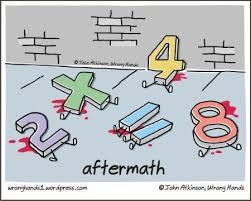
\includegraphics[width=0.35\textwidth]{aftermath.jpg}
\end{center}

Now write a 400--450 word essay addressing the following: (to be turned in the next class session)
\begin{itemize}
\item What is it that you currently do in analyzing a complicated
  mathematics problem?  
\item What elements do you look for in trying to
  gain a better understanding of a problem?  
\item What strategies would you
  recommend to someone to implement that is stuck for some time on a
  mathematics problem, irrespective of the type of math problem it is?
\item Develop your own unique list of steps and strategies that you are
  going to follow in this module when dealing with the many
  complicated math problems that you will confront.
\item Finding and receiving appropriate assistance to gain a better handle on how to tackle complicated mathematics problems is always necessary in order to improve our own problem solving abilities.  Describe how you define to be an appropriate and educationally sound use of assistance in learning how to improve your own analytical skills and problem solving strategies.
\end{itemize}
	

\begin{figure*}[h!]
  \centering
  
\includegraphics[width=0.35\textwidth]{talking-calculator.jpg}
\end{figure*}

Note that getting too much or inappropriate assistance is counterproductive to developing and improving your own skills to think about and to solve problems.  It is in the productive struggle that you learn and progress the most.  Do not cheat yourself of the opportunity to grow analytically by just trying to find solutions to problems that you yourself do not do spend the majority of the time thinking and struggling.

It is perfectly natural to feel tired, mentally drained, frustrated, even anxious about getting the answer.

The real litmus test to your overall progress is not whether you get the “correct” answer; nor is it your overall course grade or gpa.   The real measure of your success in how much you have improved in your thinking skills and how much you have learned from where you started.


So finally, include in your essay VERY specific and detailed things, that you are going to do to maximize this opportunity to learn how to be a better, more accurate and clearer thinker.

\clearpage

\begin{center}
  Homework Exercises
\end{center}

\begin{enumerate}
\item List specific things you will do to be a better math student.

  \vfill
  
\item List things you will avoid doing

  \vfill

  \clearpage

  
\item Fill in the chart below by labeling times you will study, times you will work, and times you are in class.

  \begin{figure*}[h!]
    \centering
    \rowcolors{2}{gray!25}{white}
  \begin{tabular}{|C{0.72in}|C{0.72in}|C{0.72in}|C{0.735in}|C{0.72in}|C{0.72in}|C{0.72in}|C{0.72in}|}
    \hline \rowcolor{gray!50} \textbf{Time} & \textbf{Monday} & \textbf{Tuesday} & \textbf{Wednesday} & \textbf{Thursday} & \textbf{Friday} & \textbf{Saturday} & \textbf{Sunday}\\ [0.1in] \hline
    &&&&&&&\\ [0.17in] \hline
    &&&&&&&\\ [0.17in] \hline
    &&&&&&&\\ [0.17in] \hline
    &&&&&&&\\ [0.17in] \hline
    &&&&&&&\\ [0.17in] \hline
    &&&&&&&\\ [0.17in] \hline
    &&&&&&&\\ [0.17in] \hline
    &&&&&&&\\ [0.17in] \hline
    &&&&&&&\\ [0.17in] \hline
    &&&&&&&\\ [0.17in] \hline
    &&&&&&&\\ [0.17in] \hline
    &&&&&&&\\ [0.17in] \hline
    &&&&&&&\\ [0.17in] \hline
    &&&&&&&\\ [0.17in] \hline
    &&&&&&&\\ [0.17in] \hline
    &&&&&&&\\ [0.17in] \hline
    &&&&&&&\\ [0.17in] \hline
    &&&&&&&\\ [0.17in] \hline
    &&&&&&&\\ [0.17in] \hline
    &&&&&&&\\ [0.17in] \hline
    &&&&&&&\\ [0.17in] \hline
    &&&&&&&\\ [0.17in] \hline
    &&&&&&&\\ [0.17in] \hline
    \end{tabular}
  \end{figure*}

\end{enumerate}

\end{document}

%%% Local Variables:
%%% mode: latex
%%% TeX-master: t
%%% End:
